\chapter{Model Tuning and Results}
\label{ch:tuning}

The state-space model generated in Chapter \ref{ch:sysModeling} was adjusted such that its frequency response fit the experimental frequency response. This was done by adjusting certain parameters in the model that each represented some uncertainty in the model's physical characteristics. This adjustment was first done by hand, and then repeated in a automated process through optimization.

For this chapter, unless otherwise indicated, the state-space model was generated using $n_s=2$ structural dynamic modes and $n_\text{lag}=0$ lag terms in the Roger Approximation. This was done in order to obtain a low-order model which still could accurately capture the dynamics at low frequencies, such as those in the bandwidth of the actuators.


%%%%%%%%%%%%%%%%%%%%%%%%%%%%%%%%%%%%%%%%%%%%%%%%%%%%%%%%%%%%%%%%%%%%
\section{Tuning Parameters} %%%%%%%%%%%%%%%%%%%%%%%%%%%%%%%%%%%%%%%%
%%%%%%%%%%%%%%%%%%%%%%%%%%%%%%%%%%%%%%%%%%%%%%%%%%%%%%%%%%%%%%%%%%%%

The state-space model derived in Chapter \ref{ch:sysModeling} assumes linear structural dynamics, linear aerodynamics, and thin airfoils. It also requires perfect knowledge of mode shapes. In reality, MARGE does not conform to any of these assumptions perfectly. Thus, tuning parameters were implemented in the state-space model generation script which adjusted the structural and aerodynamic modeling to compensate for these nonlinearities and inaccuracies.

The first tuning parameter is the first wing bending natural frequency $\omega_{n2}$. This quantity has a low uncertainty, but was treated as a tuning parameter for purposes of investigation.

The next tuning parameters are the damping ratios $\zeta$ for the modes. These have higher uncertainty since viscous damping is not the most physically accurate model for structural damping. Furthermore, aerodynamic damping of motions is not accounted for in the model. These can be compensated for by adjusting the damping ratios of the modes to capture all the mechanisms of damping in one place.

The next tuning parameters are the effectiveness $\tau$ of the controls. Each control surface will not be as effective as predicted by the linear aerodynamic model due to airfoil thickness, viscous effects (such as flow separation), roughness, and gaps in construction. These can be compensated for by adjusting the control effectiveness of each control surface. These tuning parameters scale the forces predicted for the control surfaces by the linear aerodynamic model.

The final tuning parameters are scaling factors $\tau_{P_{ss}}$ for each entry of $[P_{ss}]$. (Refer to Eq. \ref{eq:EOMwRoger} for the context in which $[P_{ss}]$ is used in modeling.) These scale the lift of the lifting surfaces (not including the control surfaces) to account for airfoil thickness, viscous effects, roughness, and gaps in construction.

A summary of tuning parameters and their default values (which apply no correction) is shown in Table \ref{tab:tuningParams}. The comparison of this initial un-tuned model's FRFs and the experimental FRFs can be seen in Fig. \ref{fig:noTuneFRF}.
\begin{table}[h]
	\centering
	\label{tab:tuningParams}
	\caption{Default Values of MARGE Tuning Parameters}
	\begin{tabular}{ccc}
		\hline\hline
		Name & Default Value & Description \\
		\hline
		$\omega_{n,2}$ & 1.4544 & first wing bending mode frequency \\
		$\{\zeta\}$ & $\begin{Bmatrix} 0 \\ 0.028 \end{Bmatrix}$ & modal damping ratios \\
		$\tau_\text{ail1}$ & 1 & aileron 1 effectiveness scaling \\
		$\tau_\text{ail2}$ & 1 & aileron 2 effectiveness scaling \\
		$\tau_\text{elev}$ & 1 & elevator effectiveness scaling \\
		$\tau_\text{gust}$ & 1 & gust vane effectiveness scaling \\
		$\left[\tau_{P_{ss1}}\right]$ & $\begin{bmatrix} 1 & 1 \\ 1 & 1 \end{bmatrix}$ & scaling lift from state \\
		$\left[\tau_{P_{ss2}}\right]$ & $\begin{bmatrix} 1 & 1 \\ 1 & 1 \end{bmatrix}$ & scaling lift from state rates \\
		$\left[\tau_{P_{ss3}}\right]$ & $\begin{bmatrix} 1 & 1 \\ 1 & 1 \end{bmatrix}$ & scaling lift from state accelerations \\
		\hline\hline
	\end{tabular}
\end{table}
Note that Table \ref{tab:tuningParams} applies for the case of $n_s=2$ structural dynamic modes used in modeling. When a higher number of modes is used, $\{\zeta\}$ continues to extend with damping ratios of higher modes from the GVT results (found in Table \ref{tab:expModalData}) and the Roger matrix scaling factors $[\tau_{P_{ssi}}]$ are a larger matrix of ones.

\begin{landscape}

\begin{figure}[H]
	\centering
	\label{fig:noTuneFRF}
	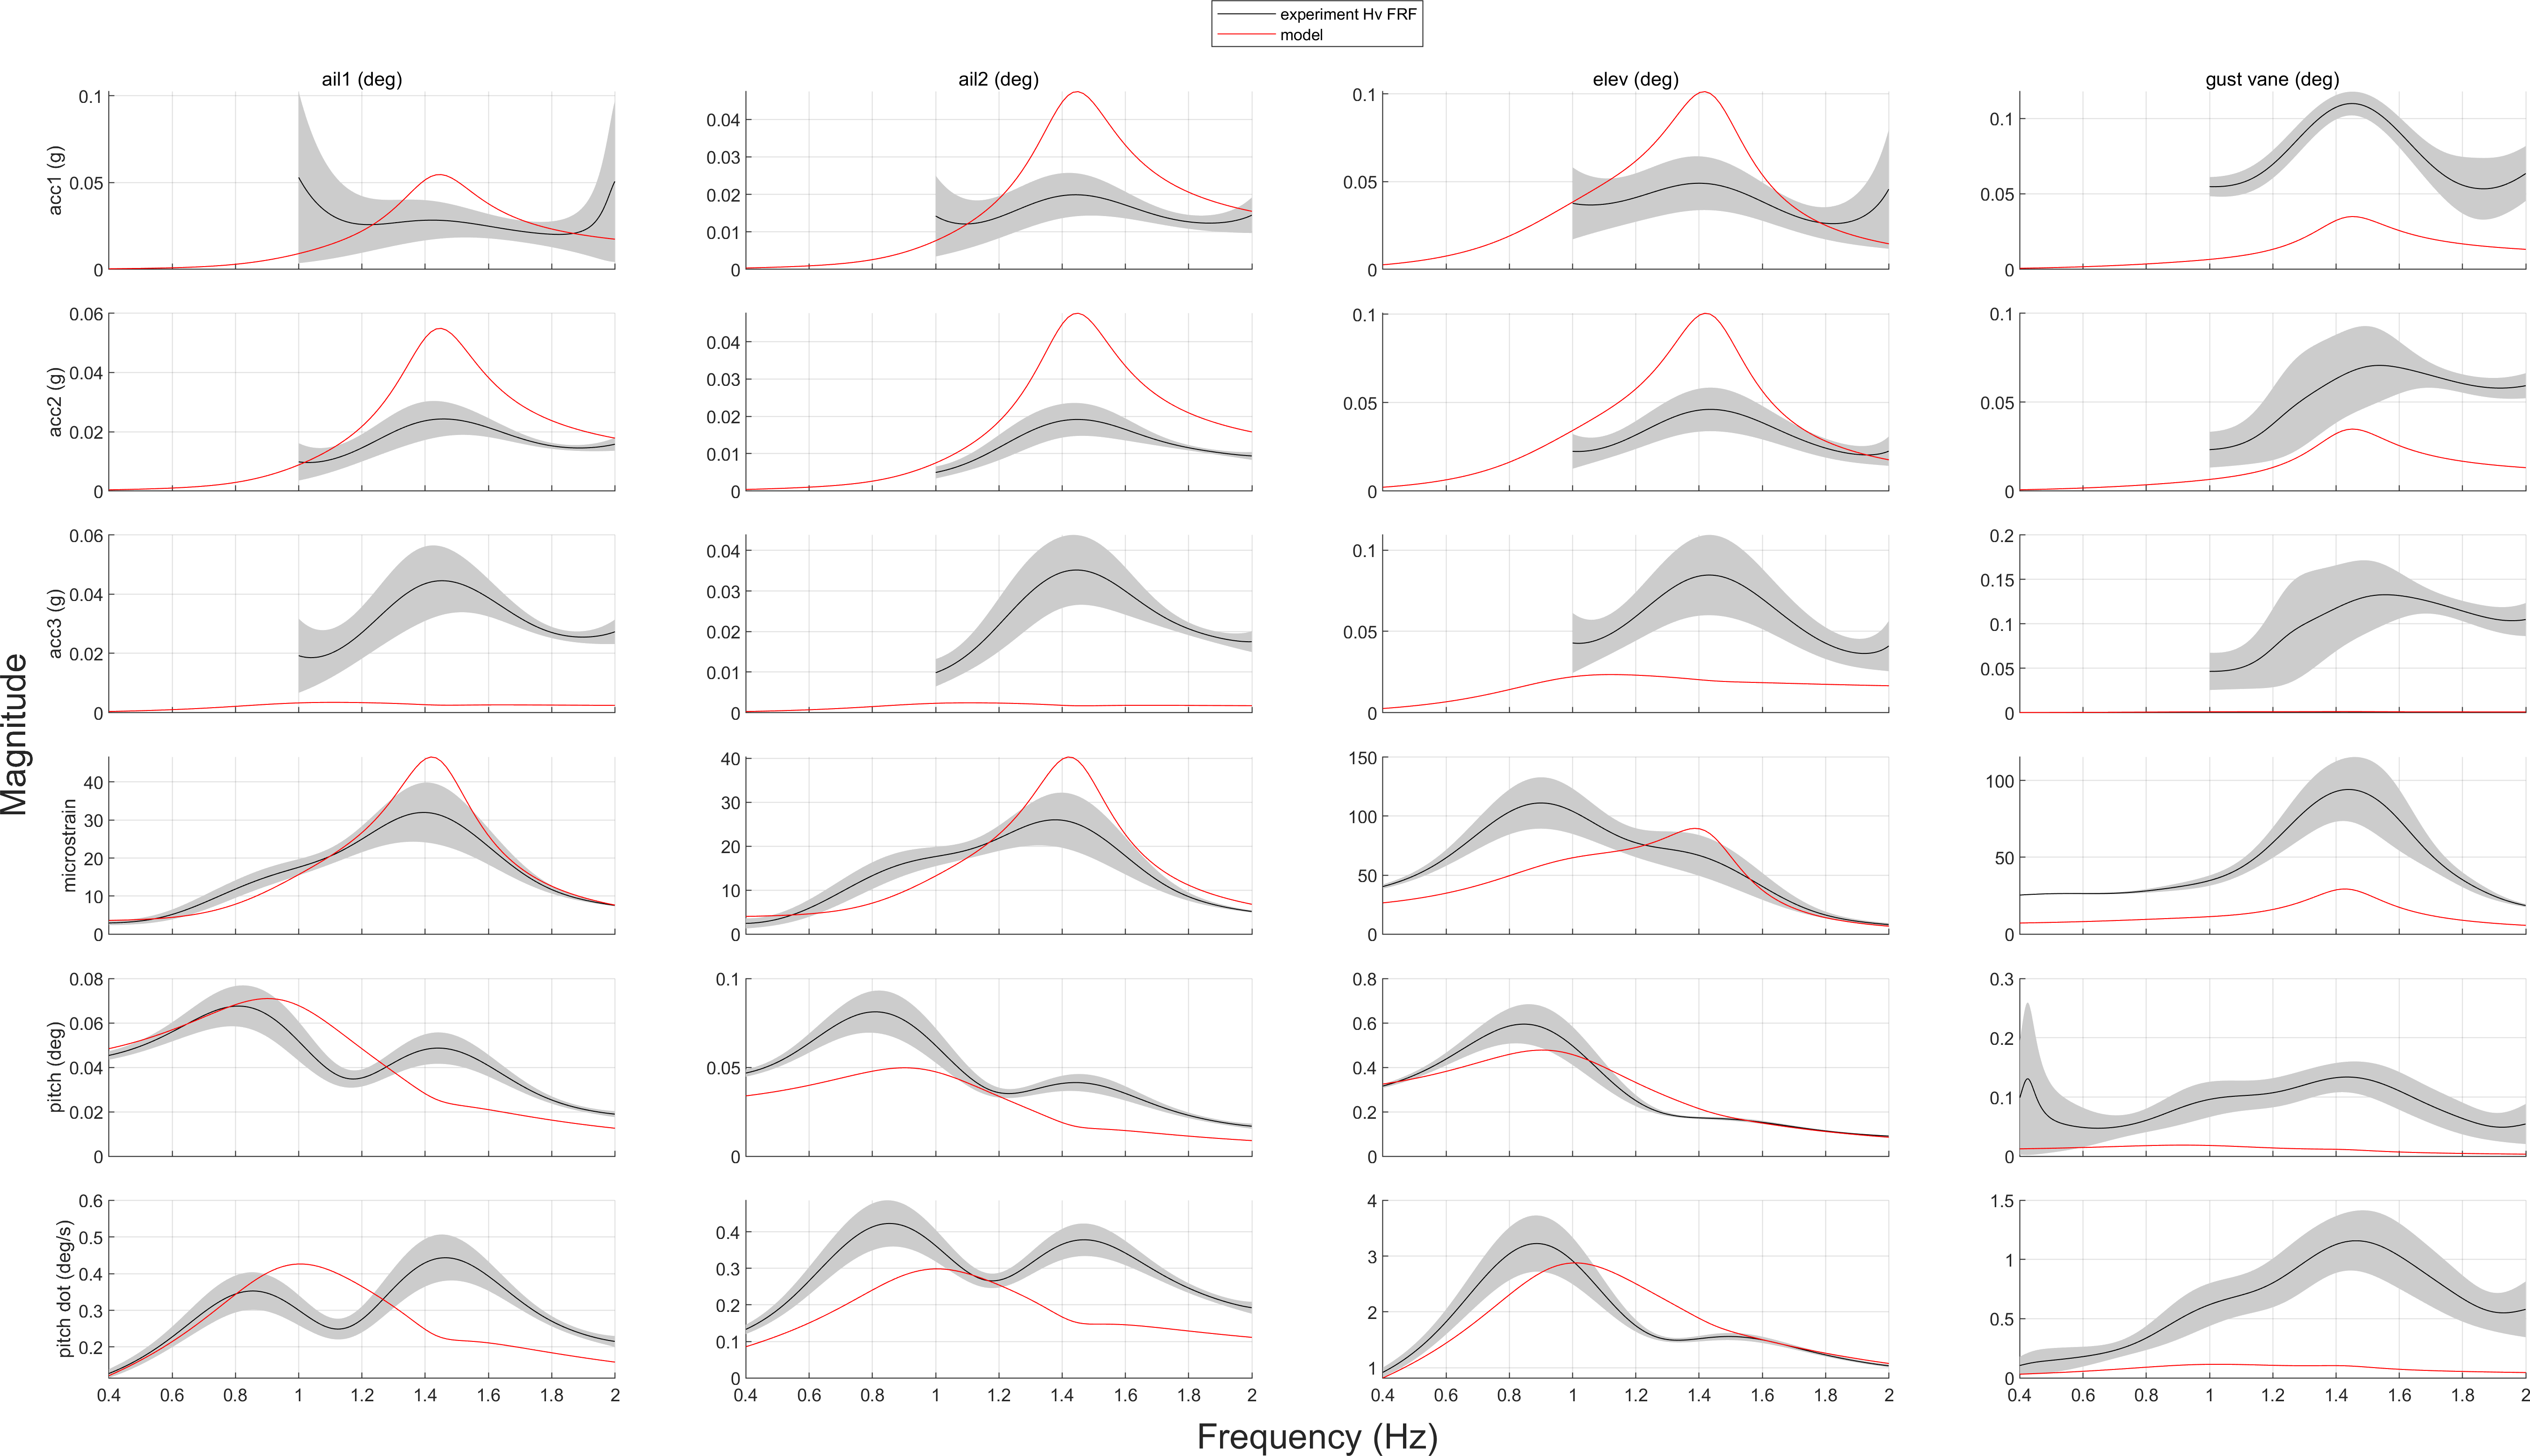
\includegraphics[width=9in]{figs/FRFcompare_noTune_q207.png}
	\caption{A comparison of experimental FRFs and untuned model FRFs at $q=207$ Pa. The grey region is enclosed by the experimental $H_1$ FRF below and the experimental $H_2$ FRF above.}
\end{figure}

\end{landscape}

%%%%%%%%%%%%%%%%%%%%%%%%%%%%%%%%%%%%%%%%%%%%%%%%%%%%%%%%%%%%%%%%%%%%
\section{Manual Model Tuning} %%%%%%%%%%%%%%%%%%%%%%%%%%%%%%%%%%%%%%
%%%%%%%%%%%%%%%%%%%%%%%%%%%%%%%%%%%%%%%%%%%%%%%%%%%%%%%%%%%%%%%%%%%%
\label{sec:manualTuning}

The first step in tuning the model was experimenting with manually tuning the parameters with the goal of closing the gap between the model's FRF and the experimental FRF at a single airspeed ($q_D=207$). This was done by thinking intuitively about the modeling uncertainties which are most likely effecting the known discrepancies in the FRFs. For example, it was known that linear aerodynamics would overpredict the control surface effectiveness by up to 50\% even in reasonably small ($<10^\circ$) deflections \cite{Young1947,Riebe1955}. Thus, the control effectiveness of the ailerons and elevator were lowered until the FRFs with these controls as inputs better matched the experimental FRFs in magnitude.

The resultant parameters and FRF comparison of the manually tuned model are shown below in Table \ref{tab:manualTuning} and Fig. \ref{fig:manualTunedFRF}. The poor alignment between the model and experiment in Fig \ref{fig:manualTunedFRF} indicates that the simple and ``intuitive'' manual tuning is not sufficient to completely match the experiment.
\begin{table}[h]
	\centering
	\label{tab:manualTuning}
	\caption{Manually Tuned Values of MARGE Tuning Parameters}
	\begin{tabular}{ccc}
		\hline\hline
		Name & Default Value & Adjusted Value \\
		\hline
		$\omega_{n,2}$ & 1.4544 & 1.4544 \\
		$\zeta_1$ & 0 & 60 \\
		$\zeta_2$ & 0.028 & 0.028 \\
		$\tau_\text{ail1}$ & 1 & 0.6 \\
		$\tau_\text{ail2}$ & 1 & 0.7 \\
		$\tau_\text{elev}$ & 1 & 0.6 \\
		$\tau_\text{gust}$ & 1 & N/A \\
		$\left[\tau_{P_{ss1}}\right]$ & $\begin{bmatrix} 1 & 1 \\ 1 & 1 \end{bmatrix}$ & $\begin{bmatrix} 0.9 & 1 \\ 0.5 & 1.5 \end{bmatrix}$ \\
		$\left[\tau_{P_{ss2}}\right]$ & $\begin{bmatrix} 1 & 1 \\ 1 & 1 \end{bmatrix}$ & $\begin{bmatrix} 0.9 & 1 \\ 0.5 & 1.5 \end{bmatrix}$ \\
		$\left[\tau_{P_{ss3}}\right]$ & $\begin{bmatrix} 1 & 1 \\ 1 & 1 \end{bmatrix}$ & $\begin{bmatrix} 0.9 & 1 \\ 0.5 & 1.5 \end{bmatrix}$ \\
		\hline\hline
	\end{tabular}
\end{table}

\begin{landscape}

\begin{figure}[H]
	\centering
	\label{fig:manualTunedFRF}
	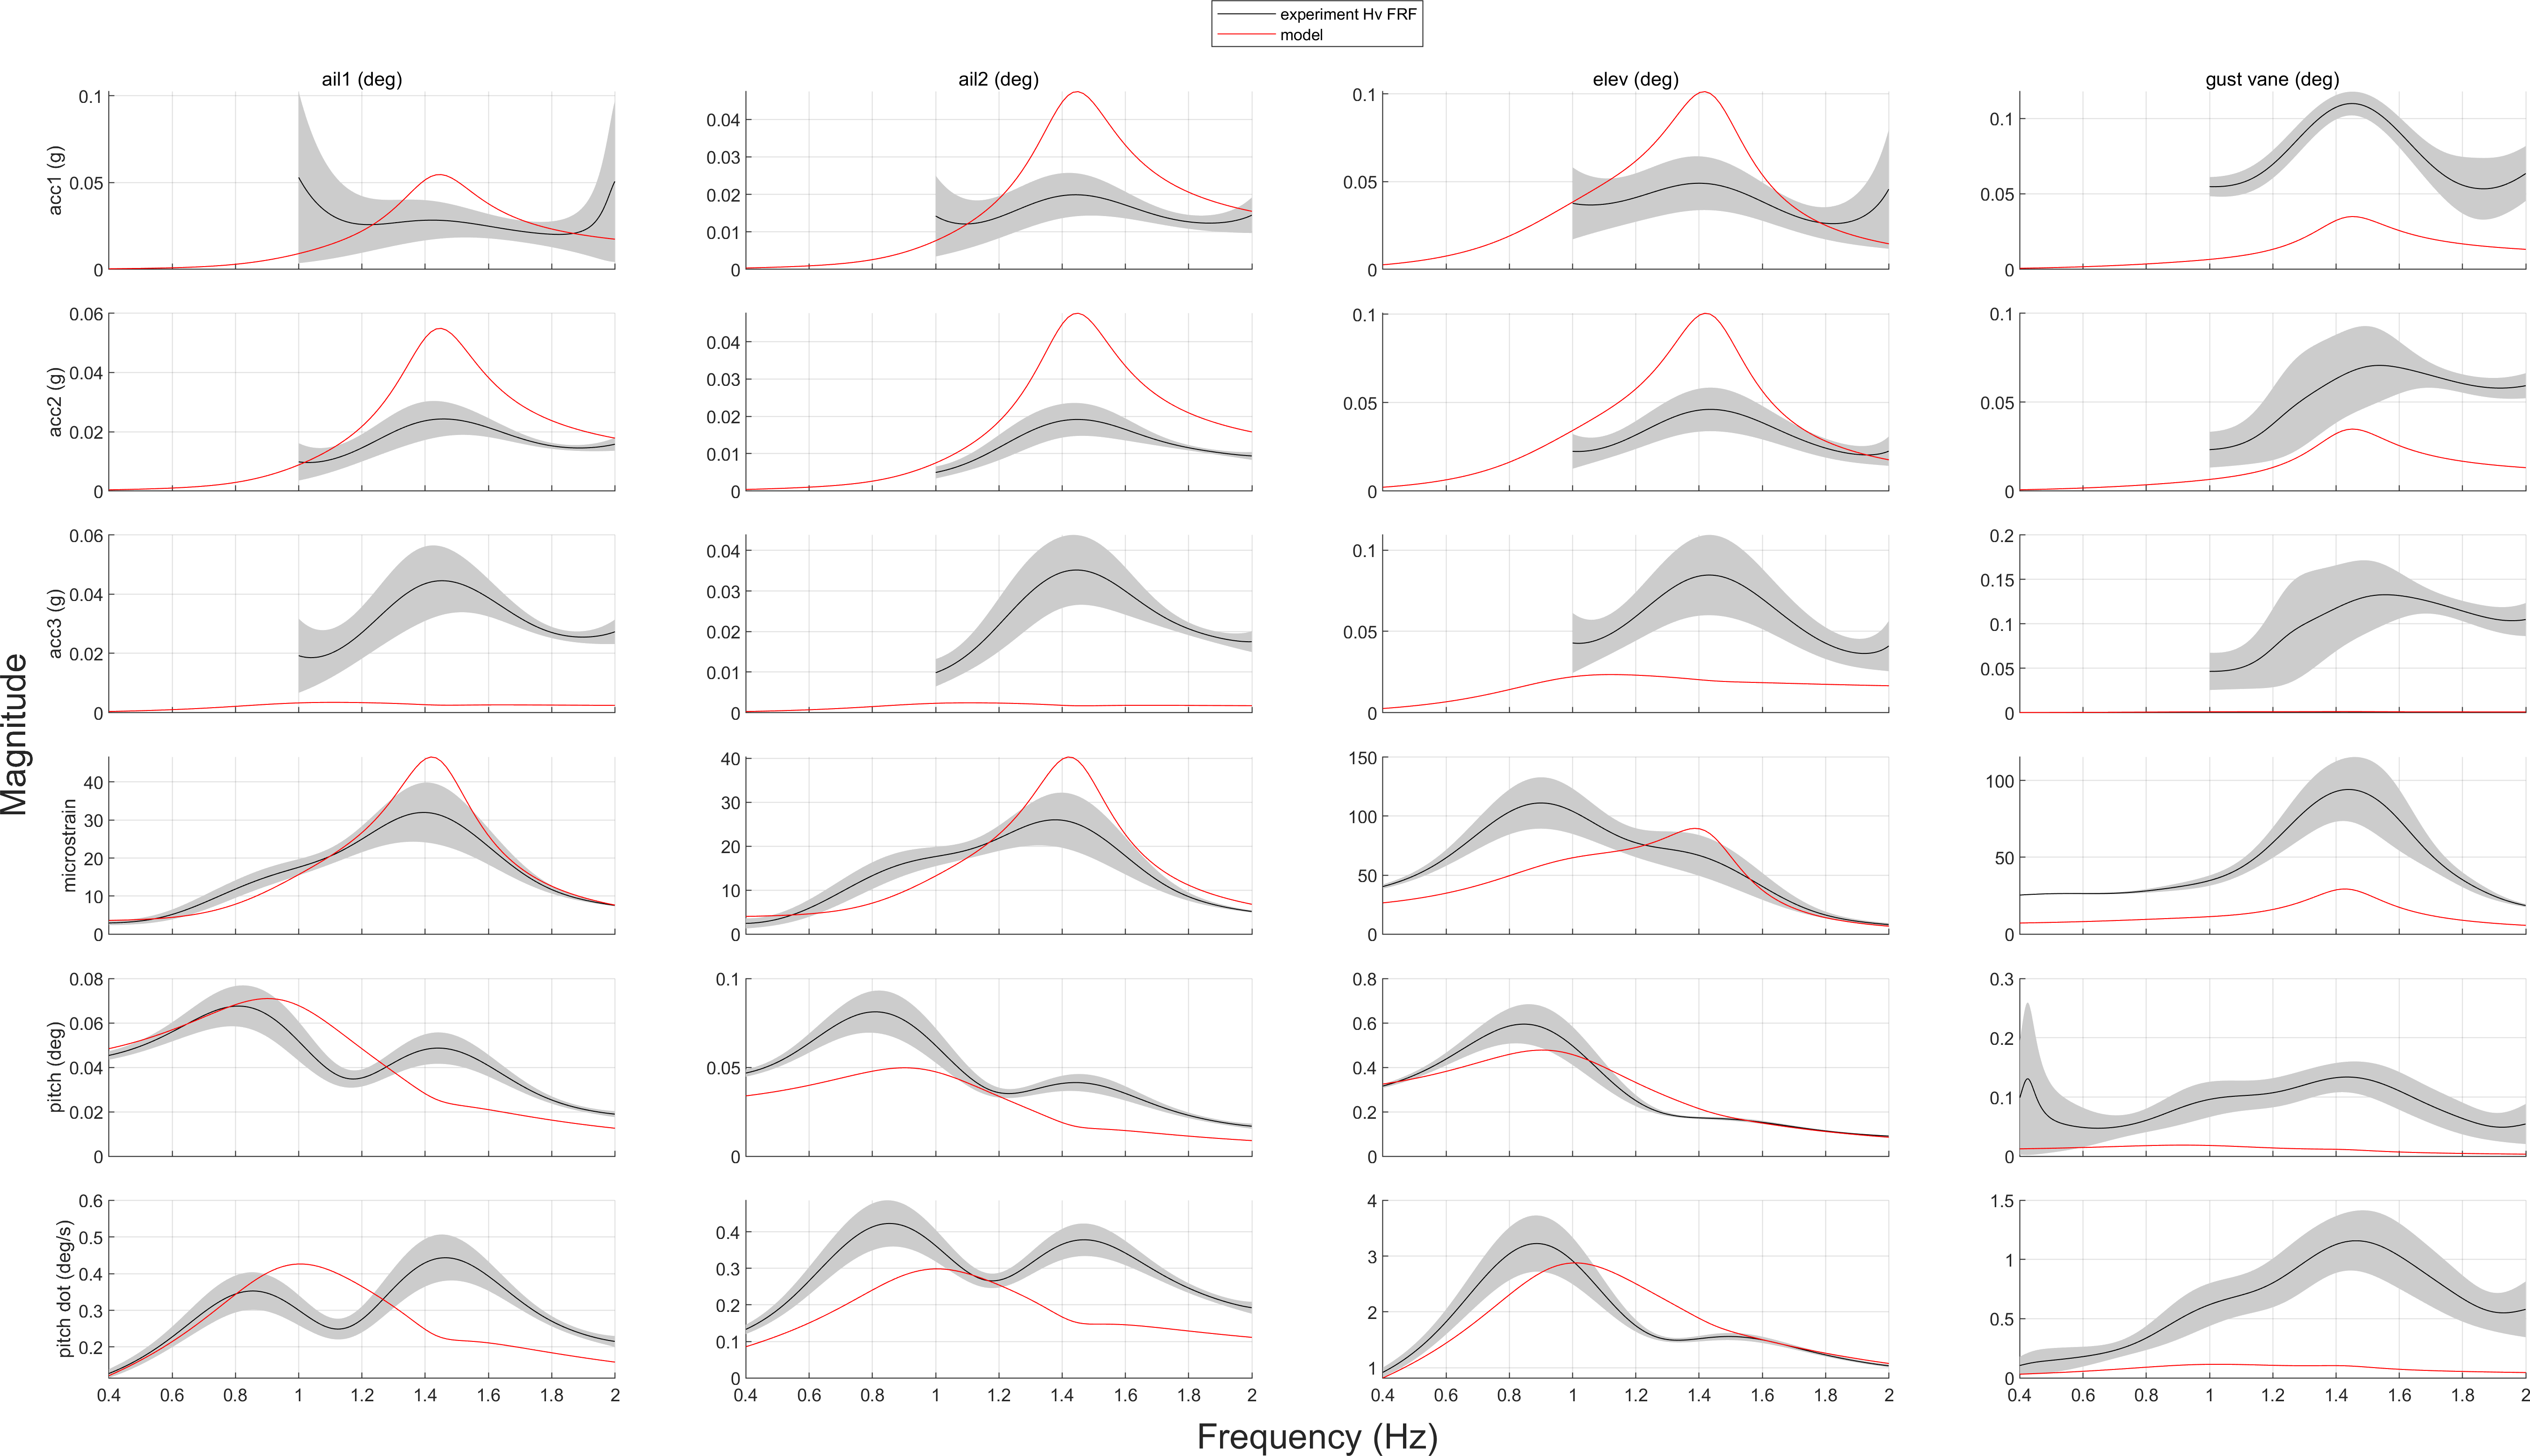
\includegraphics[width=9in]{figs/FRFcompare_manualTune_q207.png}
	\caption{A comparison of experimental FRFs and manually-tuned model FRFs. The grey region is enclosed by the experimental $H_1$ FRF below and the experimental $H_2$ FRF above.}
\end{figure}

\end{landscape}

%%%%%%%%%%%%%%%%%%%%%%%%%%%%%%%%%%%%%%%%%%%%%%%%%%%%%%%%%%%%%%%%%%%%
\section{Model Optimization} %%%%%%%%%%%%%%%%%%%%%%%%%%%%%%%%%%%%%%%
%%%%%%%%%%%%%%%%%%%%%%%%%%%%%%%%%%%%%%%%%%%%%%%%%%%%%%%%%%%%%%%%%%%%

The next step in tuning of MARGE's state-space model was to tune using optimization. Using MATLAB's \verb|fmincon| function, gradient-based optimization was used minimize the error between the model's FRFs and the experimental FRFs at all airspeeds by adjusting the tuning parameter design variables $\{x\}$ which contains the parameters listed in Table \ref{tab:tuningParams}. In order to do this, an objective function was written which would perform the following computations:
\begin{enumerate}
	\item generate MARGE's state-space model
	\item compute FRFs of the state-space model
	\item compute a scalar measure of the difference between the model's FRFs and the experimental FRFs
\end{enumerate}
The first two computations were discussed in Chapter \ref{ch:sysModeling} and Section \ref{sec:wtDAQ}.

One additional difference between the automated tuning here and the manual tuning method presented in Section \ref{sec:manualTuning} is that the FRFs involving the accelerometers were ignored in this section. This was because the results from the accelerometers were unreliable in a way that was infeasible to correct for in an automated way.

\subsubsection{Computing FRF Error} %%%%%%%%%%%%%%%%%%%%%%%%%%%%

The third computation, the scalar measure of difference between FRFs, is performed as follows:
First, the ``error'' in the magnitudes of the FRFs $\epsilon_\text{mag}$ and the ``error'' in the phase of the FRFs $\epsilon_\text{phase}$ are computed and summed across several frequencies in Eq. \ref{eq:magCompare} and \ref{eq:phaseCompare} respectively. Each difference in magnitude is normalized by the experimental magnitude at that frequency. The differences in phase are not normalized since they are already non-dimensional (in radians).
\begin{align}
	\label{eq:magCompare}
	\epsilon_{ij \, \text{mag}}(\{x\}) &= \sum_\omega \frac{|FRF_\text{exp} (\omega)| - |FRF_\text{model}(\{x\},\omega)|}{|FRF_\text{exp} (\omega)|} \\
	\label{eq:phaseCompare}
	\epsilon_{ij \, \text{phase}}(\{x\}) &= \sum_\omega \left( \angle FRF_\text{exp} (\omega) - \angle FRF_\text{model}(\{x\},\omega) \right)
\end{align}
%The actual implementation of Eq. \ref{eq:phaseCompare} is augmented with a modulo operator to take the lowest phase difference between the experimental data point and the model data point. This avoids artifacts in phase measurements due to numerical computation of phase. Thus, $\epsilon_{ij \, \text{phase}}$ is more robustly computed as
%\begin{align}
%	\epsilon_{ij \, \text{phase}} &= \sum_\omega \left( \angle FRF_\text{exp} (\omega) - \angle FRF_\text{model} (\omega)
%\end{align}
The magnitude and phase errors are then combined in a weighted sum to create the total error $f$ for an FRF. The weight $\lambda$ determines whether the error magnitude or the error in phase is more important in the optimization. This weight is set by the user.
\begin{align}
	f_{ij}(\{x\}) &= \epsilon_{ij \, \text{mag}}(\{x\}) \sqrt{\lambda} + \epsilon_{ij \, \text{phase}}(\{x\}) \frac{1}{\sqrt{\lambda}}
\end{align}
Finally the errors $f$ for each FRF (corresponding to input-output pairs) are summed to create a total error $F$ for MARGE. This is the objective function that the optimization algorithm minimizes.
\begin{align}
	F(\{x\}) &= \sum_{i=1}^{N_\text{in}} \sum_{j=1}^{N_\text{out}} f_{ij}(\{x\})
\end{align}

\subsection{Design Variable Bounds} %%%%%%%%%%%%%%%%%%%%%%%%%
The tuning parameter design variables must be optimized within a bounded domain in order to guarantee a finite and physical solution. Thus, lower and upper bounds were placed on the design variables based on physical constraints and the level of expected uncertainty in the initial value. The bounds set on the design variables are listed in Table \ref{tab:optBounds}.

Note that all damping ratios are constrained to be positive. Also, all of the aerodynamic multipliers are bounded between zero and one. This is because linear aerodynamics is expected to overpredict forces, and thus a multiplier less than one is expected.

\begin{table}[h]
	\centering
	\label{tab:optBounds}
	\caption{Bounds of MARGE Tuning Parameter Design Variables}
	\begin{tabular}{ccc}
		\hline\hline
		Name & Lower Bound & Upper Bound \\
		\hline
		$\omega_{n,2}$ & $0.9\times1.4544$ & $1.1\times1.4544$ \\
		$\zeta_1$ & 0 & $\infty$ \\
		$\zeta_2$ & $0.5\times0.028$ & $2\times0.028$ \\
		$\tau_\text{ail1}$ & 0 & 1 \\
		$\tau_\text{ail2}$ & 0 & 1 \\
		$\tau_\text{elev}$ & 0 & 1 \\
		$\tau_\text{gust}$ & 0 & 1 \\
		$\left[\tau_{P_{ss1}}\right]$ & $\begin{bmatrix} 0 & 0 \\ 0 & 0 \end{bmatrix}$ & $\begin{bmatrix} \infty & \infty \\ \infty & \infty \end{bmatrix}$ \\
		$\left[\tau_{P_{ss2}}\right]$ & $\begin{bmatrix} 0 & 0 \\ 0 & 0 \end{bmatrix}$ & $\begin{bmatrix} \infty & \infty \\ \infty & \infty \end{bmatrix}$ \\
		$\left[\tau_{P_{ss3}}\right]$ & $\begin{bmatrix} 0 & 0 \\ 0 & 0 \end{bmatrix}$ & $\begin{bmatrix} \infty & \infty \\ \infty & \infty \end{bmatrix}$ \\
		\hline\hline
	\end{tabular}
\end{table}

\subsection{Optimization Results}

A summary of the results of several model tuning optimization studies are shown in Table \ref{tab:optResult}. Each row of the table describes the parameters and the result of an optimization study.

\begin{landscape}
\begin{table}[H]
	\centering
	\label{tab:optResult}
	\caption{Model Tuning Optimization Results}
	\begin{tabular}{cccccccccc}
		\hline\hline
		\# & $n_s$ & $n_\text{lag}$ & $\lambda$ & ignore accelerometers? & $\{x_0\}$ & bounds & $\epsilon_\text{mag}(\{x\})$ & $\epsilon_\text{phase}(\{x\})$ & $F(\{x\})$ \\
		\hline
		1 & 2 & 0 & 1 & yes & default value & yes & 328 & 447 & 775 \\
		2 & 2 & 0 & 1e3 & yes & default value & yes & 282 & 519 & 8947 \\
		3 & 2 & 0 & 1e-3 & yes & default value & yes & 355 & 438 & 1386 \\
		4 & 2 & 0 & 1 & yes & manually tuned & yes & 324 & 451 & 775 \\
		5 & 2 & 0 & 1e3 & yes & manually tuned & yes & 282 & 519 & 8947 \\
		6 & 2 & 0 & 1e-3 & yes & manually tuned & yes & 358 & 416 & 1317 \\
		7 & 2 & 0 & 1 & yes & manually tuned & no & 200 & 443 & 644 \\
		8 & 2 & 0 & 1e3 & yes & manually tuned & no & 100 & 1354 & 3209 \\
		9 & 2 & 0 & 1e-3 & yes & manually tuned & no & 727 & 419 & 1326 \\
		10 & 5 & 0 & 1 & yes & manually tuned & no & 164 & 417 & 581 \\
		11 & 5 & 0 & 1e3 & yes & manually tuned & no & 124 & 1899 & 3986 \\
		12 & 5 & 0 & 1e-3 & yes & manually tuned & no & 453 & 462 & 1463 \\
		13 & 2 & 2 & 1 & yes & manually tuned & no & 144 & 414 & 559 \\
		14 & 2 & 2 & 1e3 & yes & manually tuned & no & 104 & 1622 & 3332 \\
		15 & 2 & 2 & 1e-3 & yes & manually tuned & no & 230 & 371 & 1173 \\
		13 & 5 & 2 & 1 & yes & manually tuned & no & 227 & 486 & 713 \\
		14 & 5 & 2 & 1e3 & yes & manually tuned & no & 176 & 912 & 5607 \\
		15 & 5 & 2 & 1e-3 & yes & manually tuned & no & 347 & 408 & 1292 \\
		\hline\hline
	\end{tabular}
\end{table}
\end{landscape}

%%%%%%%%%%%%%%%%%%%%%%%%%%%%%%%%%%%%%%%%%%%%%%%%%%%%%%%%%%%%%%%%
\section{Hardware Limitations} %%%%%%%%%%%%%%%%%%%%%%%%%%%%%%%%%
%%%%%%%%%%%%%%%%%%%%%%%%%%%%%%%%%%%%%%%%%%%%%%%%%%%%%%%%%%%%%%%%
\label{sec:shortcomings}


\subsection{Ground Vibration Testing}
no mode shape measurement

plastic model interferes with GVT

GVT accelerometer issues

structural damping not well-modeled

\subsection{Wind Tunnel Testing}
pitch damping in root

bad hall effect sensor

noise in accelerometers

bad data in general (visible in certain FRFs in plots)
-  john is fixing this in future with auto FRF generation and viewing